\documentclass[
11pt, % The default document font size, options: 10pt, 11pt, 12pt
%codirector, % Uncomment to add a codirector to the title page
]{charter} 



% El títulos de la memoria, se usa en la carátula y se puede usar el cualquier lugar del documento con el comando \ttitle
\titulo{Desarrollo sobre FPGA de bloque de comunicación con Sintetizador LMX2594} 

% Nombre del posgrado, se usa en la carátula y se puede usar el cualquier lugar del documento con el comando \degreename
\posgrado{Carrera de Especialización en Sistemas Embebidos} 
%\posgrado{Carrera de Especialización en Internet de las Cosas} 
%\posgrado{Carrera de Especialización en Inteligencia Artificial}
%\posgrado{Maestría en Sistemas Embebidos} 
%\posgrado{Maestría en Internet de las cosas}
% IMPORTANTE: no omitir titulaciones ni tildación en los nombres, también se recomienda escribir los nombres completos (tal cual los tienen en su documento)
% Tu nombre, se puede usar el cualquier lugar del documento con el comando \authorname
\autor{Ing. Martin Paura Bersan}

% El nombre del director y co-director, se puede usar el cualquier lugar del documento con el comando \supname y \cosupname y \pertesupname y \pertecosupname
\director{Ing. Daniel Jacoby}
\pertenenciaDirector{ITBA} 
\codirector{} % para que aparezca en la portada se debe descomentar la opción codirector en los parámetros de documentclass
\pertenenciaCoDirector{}

% Nombre del cliente, quien va a aprobar los resultados del proyecto, se puede usar con el comando \clientename y \empclientename
\cliente{BID. Erwin Beccari}
\empresaCliente{Proyecto FOCUS/UNSAM}
 
\fechaINICIO{18 de junio de 2024}		%Fecha de inicio de la cursada TSSE \fechaInicioName
\fechaFINALPlan{13 de agosto de 2024} 	%Fecha de final de cursada de TSSE
\fechaFINALTrabajo{13 de agosto de 2024}	%Fecha de defensa pública del trabajo final


\usepackage[utf8]{inputenc}
\usepackage[T1]{fontenc}
\usepackage{graphicx}
\usepackage{grffile}
\usepackage{longtable}
\usepackage{wrapfig}
\usepackage{rotating}
\usepackage[normalem]{ulem}
\usepackage{amsmath}
\usepackage{textcomp}
\usepackage{amssymb}
\usepackage{capt-of}
\usepackage{hyperref}
%\usepackage[left=2.00cm, right=2.50cm, top=2.50cm, bottom=2.00cm]{geometry}
%\usepackage{fancyhdr}
%\fancyhead[RO,LE]{\thepage}
%\fancyhead[LO]{\emph{\uppercase{\leftmark}}}
%\fancyfoot{}
%\renewcommand{\headrulewidth}{1.0pt}
%\pagestyle{fancy}
%\date{}
\title{Desarrollo sobre FPGA de tecnología SAR para constelación satelital}
\hypersetup{
 pdfauthor={},
 pdftitle={IEEE-830},
 pdfkeywords={},
 pdfsubject={},
 pdfcreator={Emacs 26.2 (Org mode 9.1.9)}, 
 pdflang={English}}


\begin{document}



\maketitle

\pagebreak 

\section*{Historial de cambios}
\label{sec:registro}


\begin{table}[ht]
\label{tab:registro}
\centering
\begin{tabularx}{\linewidth}{@{}|c|X|c|@{}}
\hline
\rowcolor[HTML]{C0C0C0} 
Revisión & \multicolumn{1}{c|}{\cellcolor[HTML]{C0C0C0}Detalles de los cambios realizados} & Fecha      \\ \hline
A      & Creación del documento                  &\fechaInicioName \\ \hline
B      & Primera entrega  & {13} de {Agosto} de 2024 \\ \hline
%2      & Se completa hasta el punto 9 inclusive	& {19} de {marzo} de 2024 \\ \hline
%3      & Se agregan puntos 11 y 12 inclusive	& {26} de {marzo} de 2024 \\ \hline
%3.1      & Se completa hasta el punto 12 inclusive	& {31} de {marzo} de 2024 \\ \hline
%4      & Se completa el plan	                                 & {2} de {abril} de 2024 \\ \hline
%4.1    & Se completa el plan con correcciones                    & {15} de {abril} de 2024 \\ \hline

% Si hay más correcciones pasada la versión 4 también se deben especificar acá

\end{tabularx}
\end{table}

\pagebreak 


\tableofcontents

\newpage

\section{Introducción}
\label{sec:org60390fa}

El presente documento detallará todos los aspectos relacionados con las especificaciones del proyecto "\ttitle ".
El objetivo del proyecto es desarrollar un módulo de comunicación SPI entre la lógica programable de la plataforma de desarrollo Arty Z7 y el Sintetizador basado en el integrado LMX2595.

\subsection{Contenido}
\label{sec:org434c3ef}

Los contenidos del presente Informe son:
\begin{enumerate}
	 \item Breve explicación de lo implementado.
	 \item Diagrama de flujo de la Maquina de Estado.
	 \item Diagrama Bloque de los módulos desarrollados/utilizados.
	 \item Simulaciones.
	 \item Tabla de uso de los recursos de la FPGA.
\end{enumerate}


\subsection{Definiciones, Acrónimos y Abreviaturas}
\label{sec:orgb158e36}

\begin{enumerate}
\item HW	Hardware
\item FW	Firmware
\item SW 	Software
\item FOCUS Emprendimiento y proyecto del sistema general.
\item HDL 	\textit{Hardware Description Language} 
\item N/A 	No aplica 
\item RADAR	\textit{RAdio Detection And Ranging}
\item SDR 	\textit{Software Defined Radio}
\item SAR	\textit{Synthetic Aperture Radar}
\item UART 	\textit{Universal Asynchronous Receiver Transmitter} 
\item FPGA 	\textit{Field Programmable Gate Array} 
\item AXI 	\textit{Advanced eXtensible Interface} 
\item RAM 	\textit{Random Access Memory}
\item HBC	\textit{High-Bandwidth Connectivity}
\end{enumerate}


%En esta subsección se definirán todos los términos, acrónimos y
%abreviaturas utilizadas en la ERS.


\subsection{Referencias}
\label{sec:org62711e0}

\begin{enumerate}
\item [1]LMX2594 Evaluation board user manual.
\item [2]LMX2594 Datasheet.
\end{enumerate}



\section{Breve explicación de lo implementado}
\label{sec:orgc1c4017}

El objetivo del proyecto final de la especialización consta de la implementación de un procesador de imagenes SAR sobre FPGA.
El mismo debe ser capaz de comunicarse con el sintetizador (que se encarga de emitir las señales de radar con frecuencia variable), la antena receptora (LP Filter) que envía una señal analógica de las señales recibidas (reflejadas en la superficie) y el GPSRTK que informa la posición actual del módulo.
Posteriormente, debe procesar la información captada y generar una imagen SAR que será transmitida a la computadora central del satélite.


\begin{figure}[htpb]
\centering 
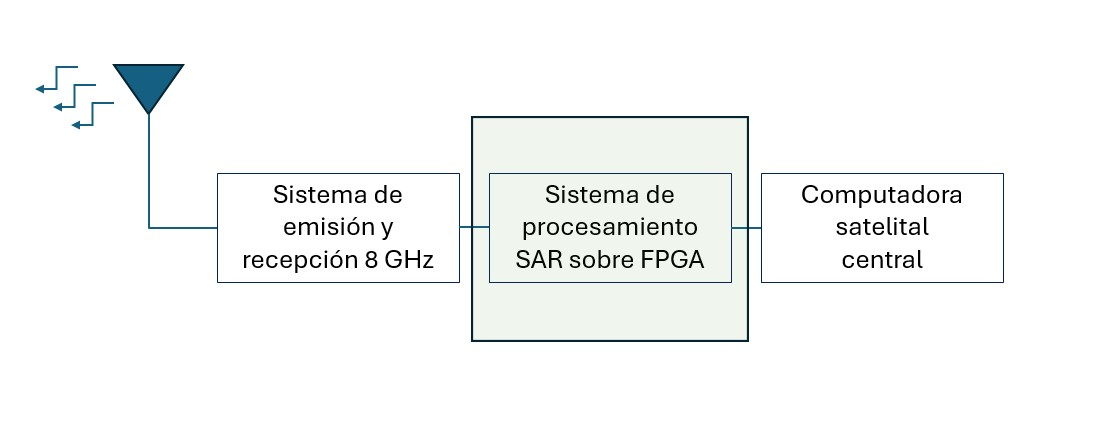
\includegraphics[width=.95\textwidth]{./Figuras/Diagrama Bloque Sistema.jpg}
\caption{Diagrama en bloques del sistema SAR.}
\label{fig:diagBloques}
\end{figure}

\vspace{25px}

Para llevar a cabo lo antes mencionado se seleccionaron distintos protocolos de comunicación entre los equipamientos como se muestra en la Figura 2.
Como alcance del proyecto final de la materia "Circuitos Lógicos Programables" se desarrollo el sistema de comunicación entre la FPGA y El sintetizador. Este último utiliza el integrado LMX2594, el cual recibe las instrucciones de configuración mediante SPI, una señal de inicio de rampa para el barrido en frecuencia de la señal emitida (SYNC 5Khz) y un clk de 100 Mhz para el funcionamiento interno.

\newpage 

\begin{figure}[htpb]
\centering 
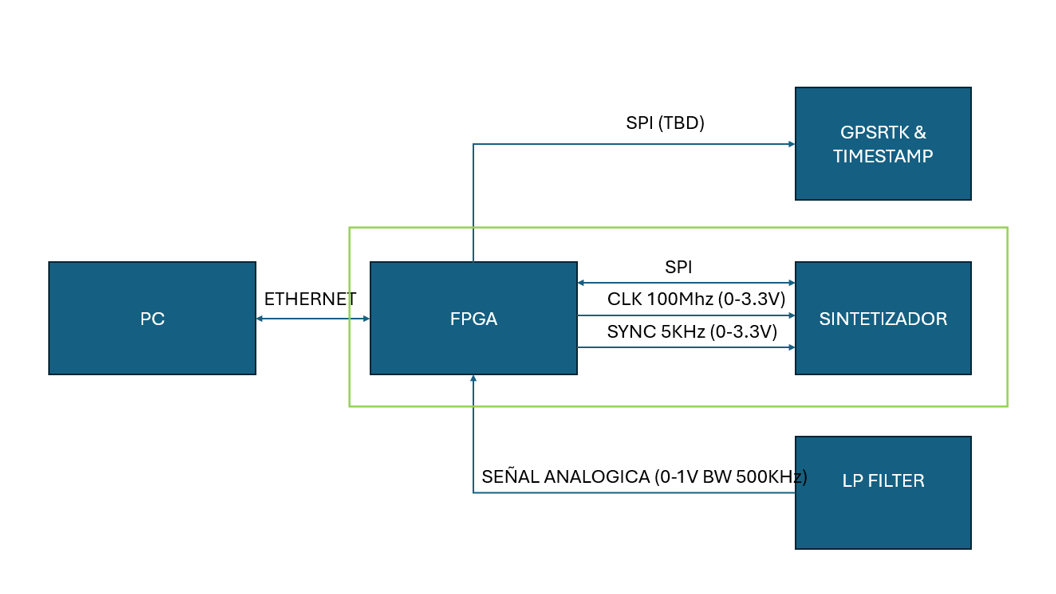
\includegraphics[width=.95\textwidth]{./Figuras/DiagramaBloquesProyecto.png}
\caption{Diagrama en bloques del proyecto CLP.}
\label{fig:diagBloques}
\end{figure}

\vspace{25px}


Para ello se desarrollo un modulo SPI que recibe las señales de control, Direccionamiento, Datos de Salida, Dato de Entrada y Señal de Final de Comunicación.

\begin{enumerate}
	\item rst: Activo alto, Resetea el módulo.
	\item ena: Activo alto, Inicia la secuencia de Comunicación.   
	\item clk\_in: Activo alto, ingreso reloj de referencia.
	\item PrescaleFactor: Natural, factor de división entre el reloj de ingreso y el utilizado para la comunicación.
	\item csb: Activo bajo, Selector de dispositivo de comunicación SPI.   
	\item sclk: Reloj de comunicación SPI (los datos se toman en el flanco ascendente).  
	\item sdat: Activo alto, Datos transmitidos desde el módulo (FPGA) al sintetizador LMX2594.   
	\item smux: Activo alto, Datos transmitidos desde el sintetizador LMX2594 al módulo (FPGA). 
	\item r\_nw: Read-Not Write, selector de modo escritura (low) o lectura (high).
	\item addr: Direccion del registro al que se desea ingresar datos o leer valor actual.
	\item data\_tx: Dato a ser cargados en el sintetizador.
	\item data\_rx: Datos a ser leídos por el módulo(FPGA).
	\item cc: Activo alto, Inidicador de final de secuencia de comunicación.
\end{enumerate}

Para las pruebas de funcionamiento del módulo se utilizo el puerto serial virtual del process system, y este posteriormente mediante los AXI BUS se comunicaban con el modulo SPI implementado el la lógica programable para transmitir los datos recibidos.



\section{Diagrama de flujo de la Maquina de Estado.}
\label{sec:orgfd5391f}

\begin{figure}[htpb]
\centering 
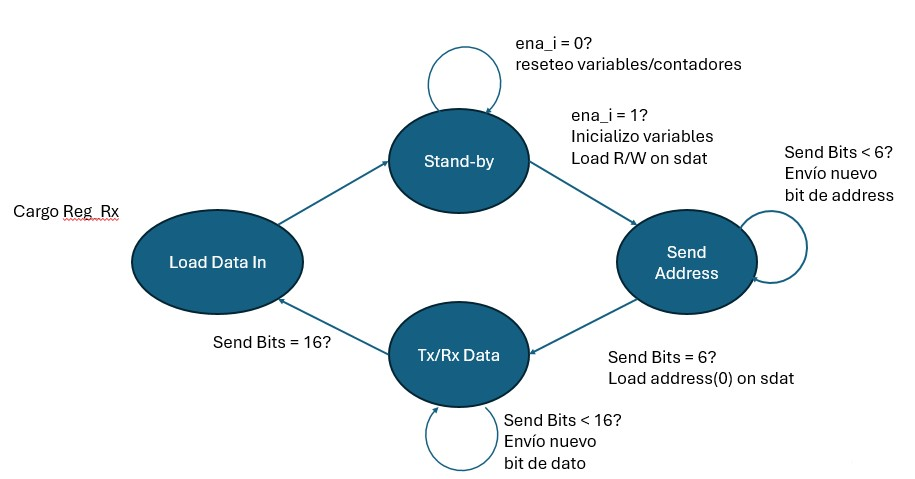
\includegraphics[width=.95\textwidth]{./Figuras/MaqEstSPI.jpg}
\caption{Diagrama Maquina de Estados SPI.}
\label{fig:diagBloques}
\end{figure}

\vspace{25px}

\section{Diagrama Bloque de los módulos desarrollados/utilizados}
\label{sec:org307bb59}

\begin{figure}[htpb]
\centering 
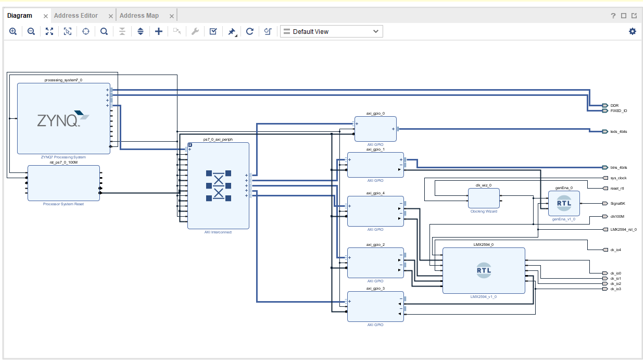
\includegraphics[width=.95\textwidth]{./Figuras/Diagramaenbloquesgeneral.png}
\caption{Diagrama en Bloque General de la implementación (PS y PL).}
\label{fig:diagBloques}
\end{figure}

\vspace{25px}

\begin{figure}[htpb]
\centering 
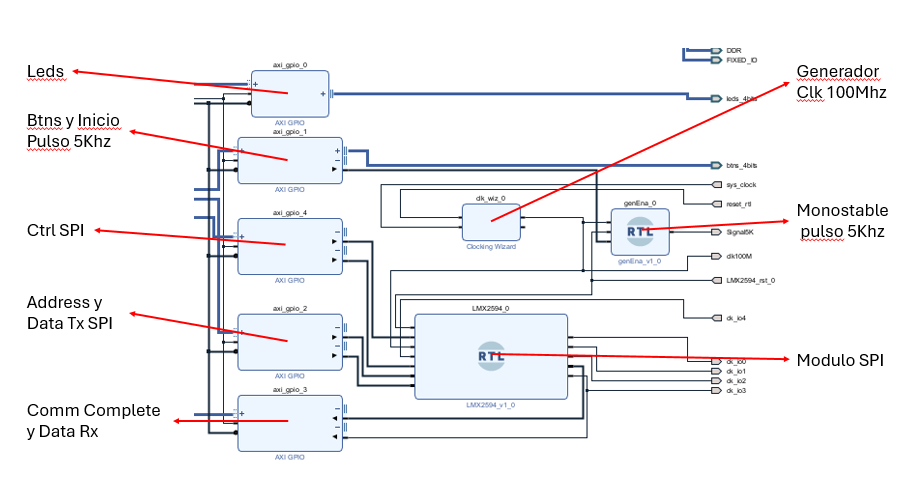
\includegraphics[width=.95\textwidth]{./Figuras/Descripciónbloques.png}
\caption{Bloques implementados para CLP (AXI y PL).}
\label{fig:diagBloques}
\end{figure}

\vspace{25px}


\section{Simulaciones}
\label{sec:org49fe900}

A continuación, el la Figura [6] se muestra una simulación conciderando un puente entre el puerto de salida de datos seriales y el puerto de ingreso.
En la primer trama el dato enviado es 0x5555, y al final de la comunicación el registro de entrada toma ese valor. En la segunda trama se envía el dato 0xAAAA y se observa que al final de la comunicación el valor del dato leido es el mismo, 0xAAAA.

\begin{figure}[htpb]
\centering 
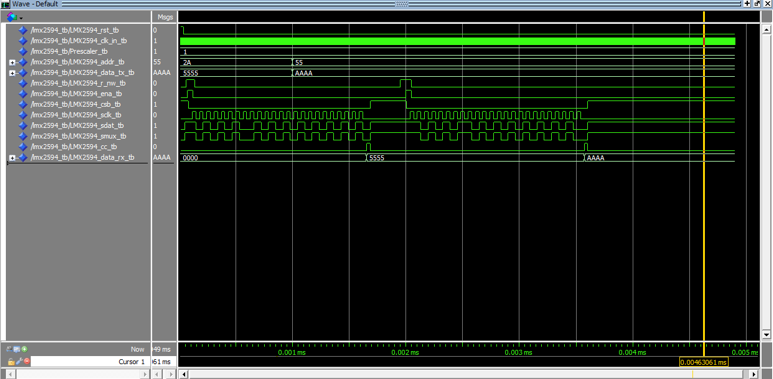
\includegraphics[width=.95\textwidth]{./Figuras/SimulaciónModelSim.png}
\caption{Simulación con puente entre el puerto de entrada y salida de datos.}
\label{fig:diagBloques}
\end{figure}

\vspace{25px}

Mediciones realizadas en laboratorio de la salida de los puertos de a FPGA. Se envian datos mediante el puerto serial al PS y estos datos son reenviados mediante el módulo SPI.


\begin{figure}[htpb]
\centering 
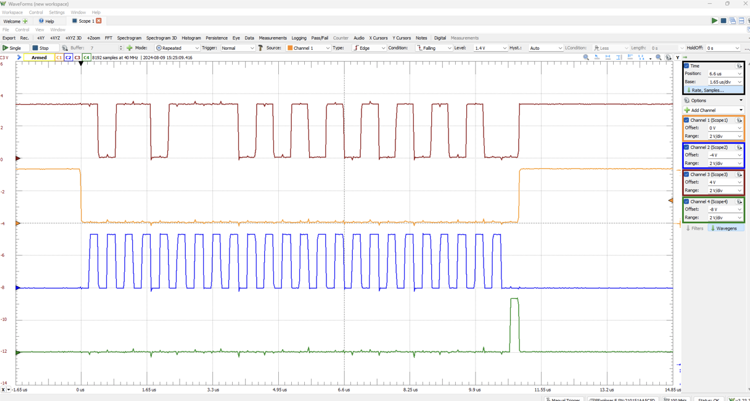
\includegraphics[width=.95\textwidth]{./Figuras/SeñalesTx1.png}
\caption{Mediciones R/W=Read; Add=0x6F(‘o’); Data=0xAA}
\label{fig:diagBloques}
\end{figure}

\vspace{25px}

\begin{figure}[htpb]
\centering 
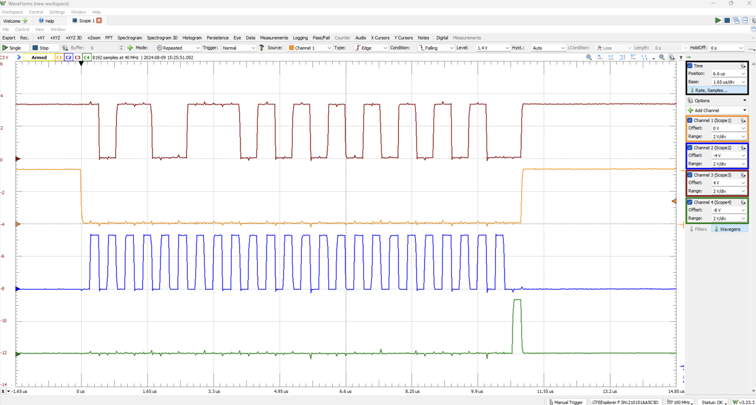
\includegraphics[width=.95\textwidth]{./Figuras/SeñalesTx67.png}
\caption{Mediciones R/W=Read; Add=0x67(‘g’); Data=0xAA}
\label{fig:diagBloques}
\end{figure}

\vspace{25px}


\begin{figure}[htpb]
\centering 
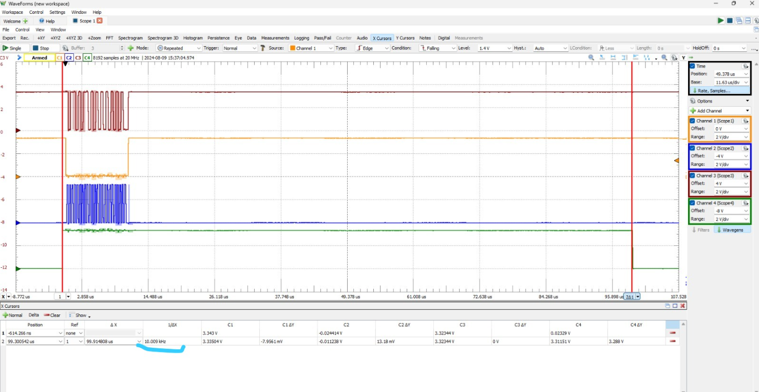
\includegraphics[width=.95\textwidth]{./Figuras/SeñalesTxy5K.png}
\caption{Mediciones R/W=Read; Add=0x35(‘5’)= orden de disparo señal Sync 5Khz; Data=0xAA}
\label{fig:diagBloques}
\end{figure}

\vspace{25px}

\newpage

\section{Tabla de uso de los recursos de la FPGA}
\label{sec:orgd0babc0}

\begin{figure}[htpb]
\centering 
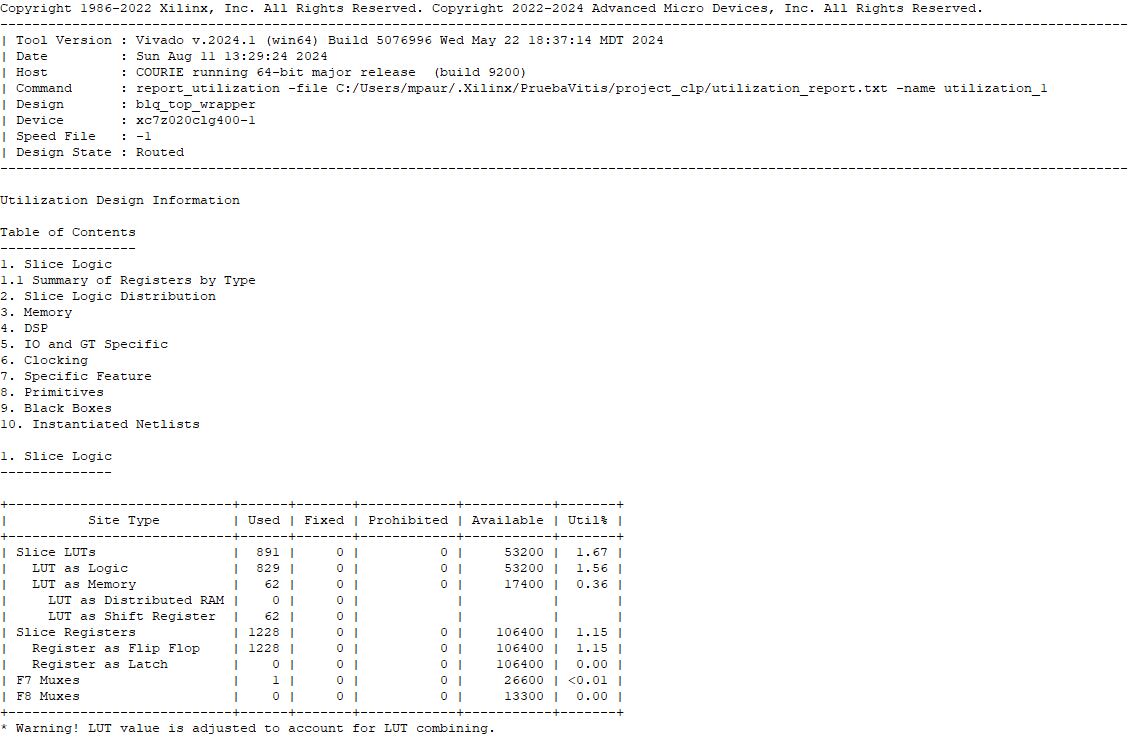
\includegraphics[width=.95\textwidth]{./Figuras/SliceLogic.png}
\end{figure}

\begin{figure}[htpb]
\centering 
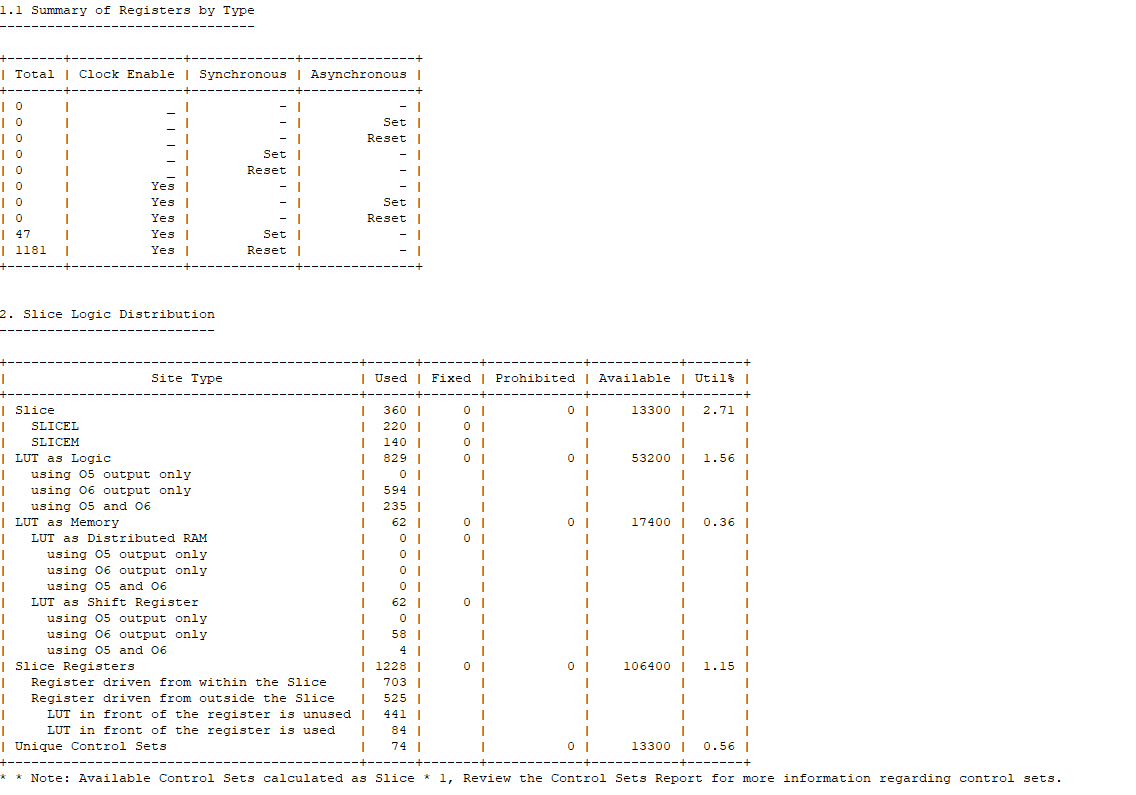
\includegraphics[width=.95\textwidth]{./Figuras/SummaryRegType.png}
\end{figure}

\begin{figure}[htpb]
\centering 
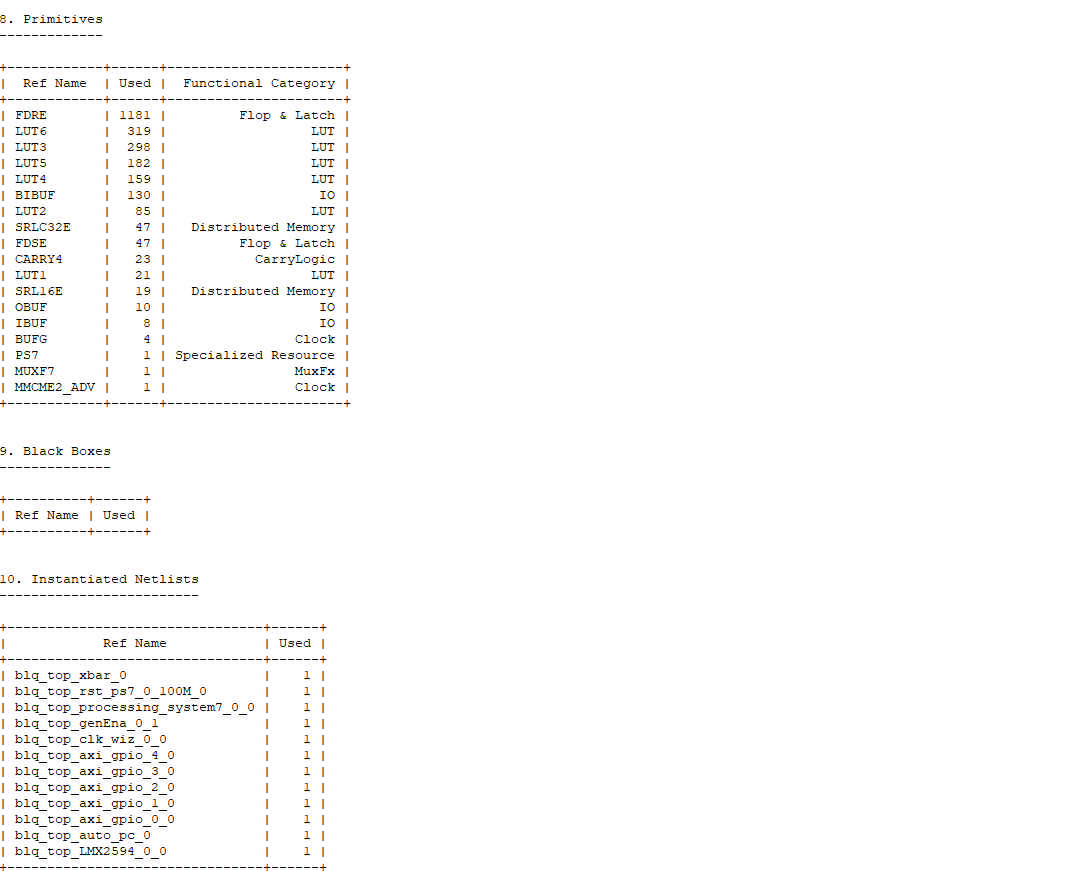
\includegraphics[width=.95\textwidth]{./Figuras/Primitives.png}
\end{figure}


\begin{figure}[htpb]
\centering 
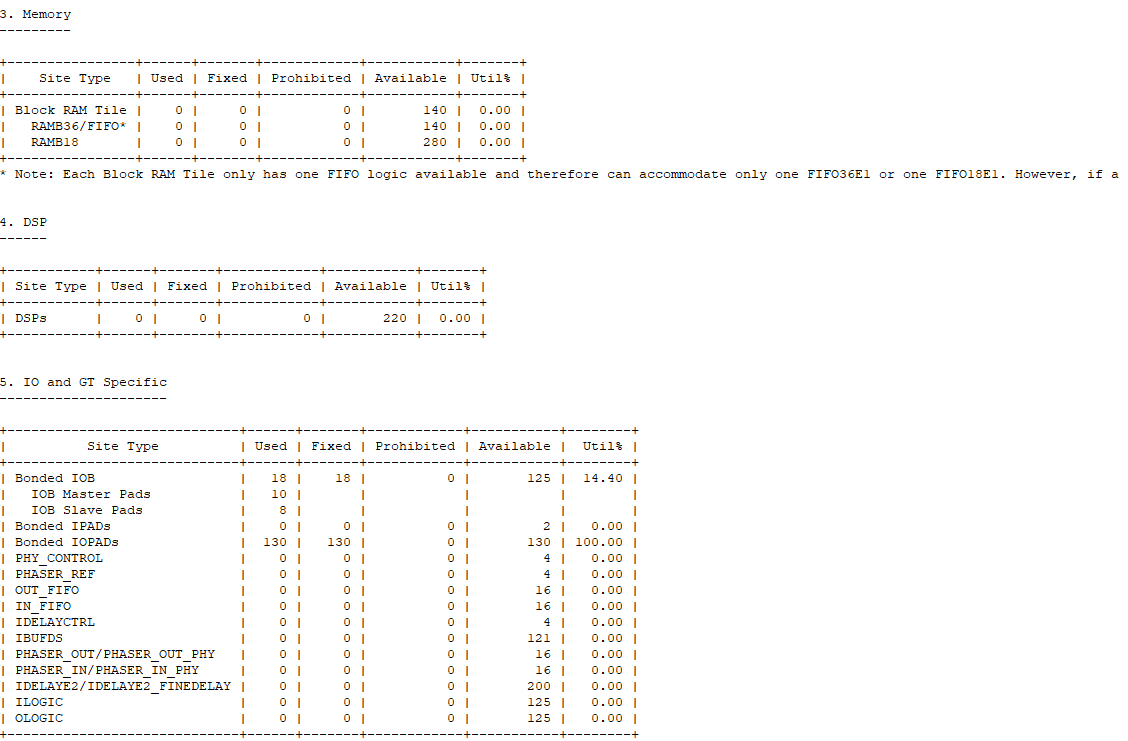
\includegraphics[width=.95\textwidth]{./Figuras/MemoryDSP.png}
\end{figure}




\end{document}
